%%&program=xelatex
%&encoding=UTF-8 Unicode
% SVN keywords
% $Author: bernardo $
% $Date: 2014-10-24 15:26:00 +0100 (Fri, 24 Oct 2014) $
% $Revision: 6732 $
% $URL: http://metis.ipfn.ist.utl.pt/svn/cdaq/Users/Bernardo/Aulas/LFEB/teXfiles/ContrucoesGeometrica/ConstrucoesGeomet.tex $
\documentclass[a4paper,12pt]{article}      % Comments after  % are ignored
%\usepackage{hyperref}                 % For creating hyperlinks in cross references
%
%MUDAR procedimento lente divergente + angulo de Brewster
\usepackage{ifxetex}% for XELATEX, or PDFlatex
\usepackage{ifplatform} 
%
\ifxetex
	\usepackage{polyglossia} \setmainlanguage{portuges}
	\usepackage{fontspec}
	\ifwindows
		\setmainfont[Ligatures=TeX]{Garamond}
		\setsansfont[Ligatures=TeX]{Gill Sans MT}
		\setmonofont{Consolas}		
%		\setmonofont[Scale=MatchLowercase]{Courier}
	\fi
	\iflinux
		\setmainfont[Ligatures=TeX]{Linux Libertine O}
		\setsansfont[Ligatures=TeX,Scale=MatchLowercase]{Linux Biolinum}
		\setmonofont[Scale=MatchLowercase]{Courier}
	\fi
	\ifmacosx
	% add settings
	% Use xelatex -no-shell ...
		\setmainfont[Ligatures=TeX]{Garamond}
		\setsansfont[Ligatures=TeX]{Helvetica}
		\setmonofont{Consolas}
	\fi
	\usepackage{xcolor,graphicx} 
\else
	\usepackage[portuguese]{babel}
	%\usepackage[latin1]{inputenc}
	\usepackage[utf8]{inputenc}
	\usepackage[T1]{fontenc}
	\usepackage{graphics}                 % Packages to allow inclusion of graphics
	\usepackage{color}                    % For creating coloured text and background
\fi

\usepackage{enumitem}
\setlist{nolistsep}

\usepackage{tikz}
%\usetikzlibrary{calc,arrows,decorations.pathmorphing,intersections}


\usepackage{amsmath,amssymb,amsfonts} % Typical maths resource packages
\usepackage[retainorgcmds]{IEEEtrantools}

\oddsidemargin 0cm
\evensidemargin 0cm

\pagestyle{myheadings}         % Option to put page headers
                               % Needed \documentclass[a4paper,twoside]{article}
\markboth{{\small \it  Laboratório de Física Experimental Básica}}
{{\small\it MEFT - 1º Sem. 2014/2015} }

\addtolength{\hoffset}{-0.5cm}
\addtolength{\textwidth}{2.5cm}
\addtolength{\topmargin}{-1.5cm}
\addtolength{\textheight}{3cm}

%\textwidth 15.5cm
%\topmargin -1.5cm
\setlength{\parindent}{0pt}
\setlength{\parskip}{1ex  plus  0.5ex  minus  0.2ex}
%\parindent 0.5cm
%\textheight 25cm
%\parskip 1mm


% Math macros
\newcommand{\ud}{\,\mathrm{d}} 
\newcommand{\HRule}{\rule{\linewidth}{0.5mm}}

\author{Prof. Bernardo B. Carvalho} 

%%%%, Bernardo Brotas Carvalho\\bernardo@ipfn.ist.utl.pt} 
\date{ Outubro 2012} 

\begin{document} 

	
\includegraphics[width=0.2\textwidth]{../logo-ist}%\\[1cm]  %%  Logo_IST_color

	\HRule \\[0.5cm]
	{ \huge \sf  \textsc{Instrumentos Óticos Simples e Goniómetro}} \\[0.4cm] % \bfseries 
%	{ \huge \sf  \textsc{Sistemas ótipos baseados em Lentes Delgadas e aproximação paraxial} }\\[0.4cm] % \bfseries 
%	{ \large \bfseries Construções Geométricas em Lentes Delgadas %(aproximação paraxial)}\\
%	{ \large \bfseries Procedimento Experimental}\\
	\HRule \\%[0.5cm]

%\newpage
\section{\sf Protocolo Experimental}
\subsection{\sf Introdução}
Pretende-se com este trabalho desenhar e montar no laboratório montagem ou sistemas óticos compostos com duas ou mais lentes delgadas testando as suas características principais. As duas montagens, um telescópio simples e um microscópio são variações do esquema ótico apresentado na secção 2.5.1 do Trabalho de Ótica Geométrica (ver Figura \ref{fig:Telescopio}). 

\begin{figure}
	[!htb]  \centering 
	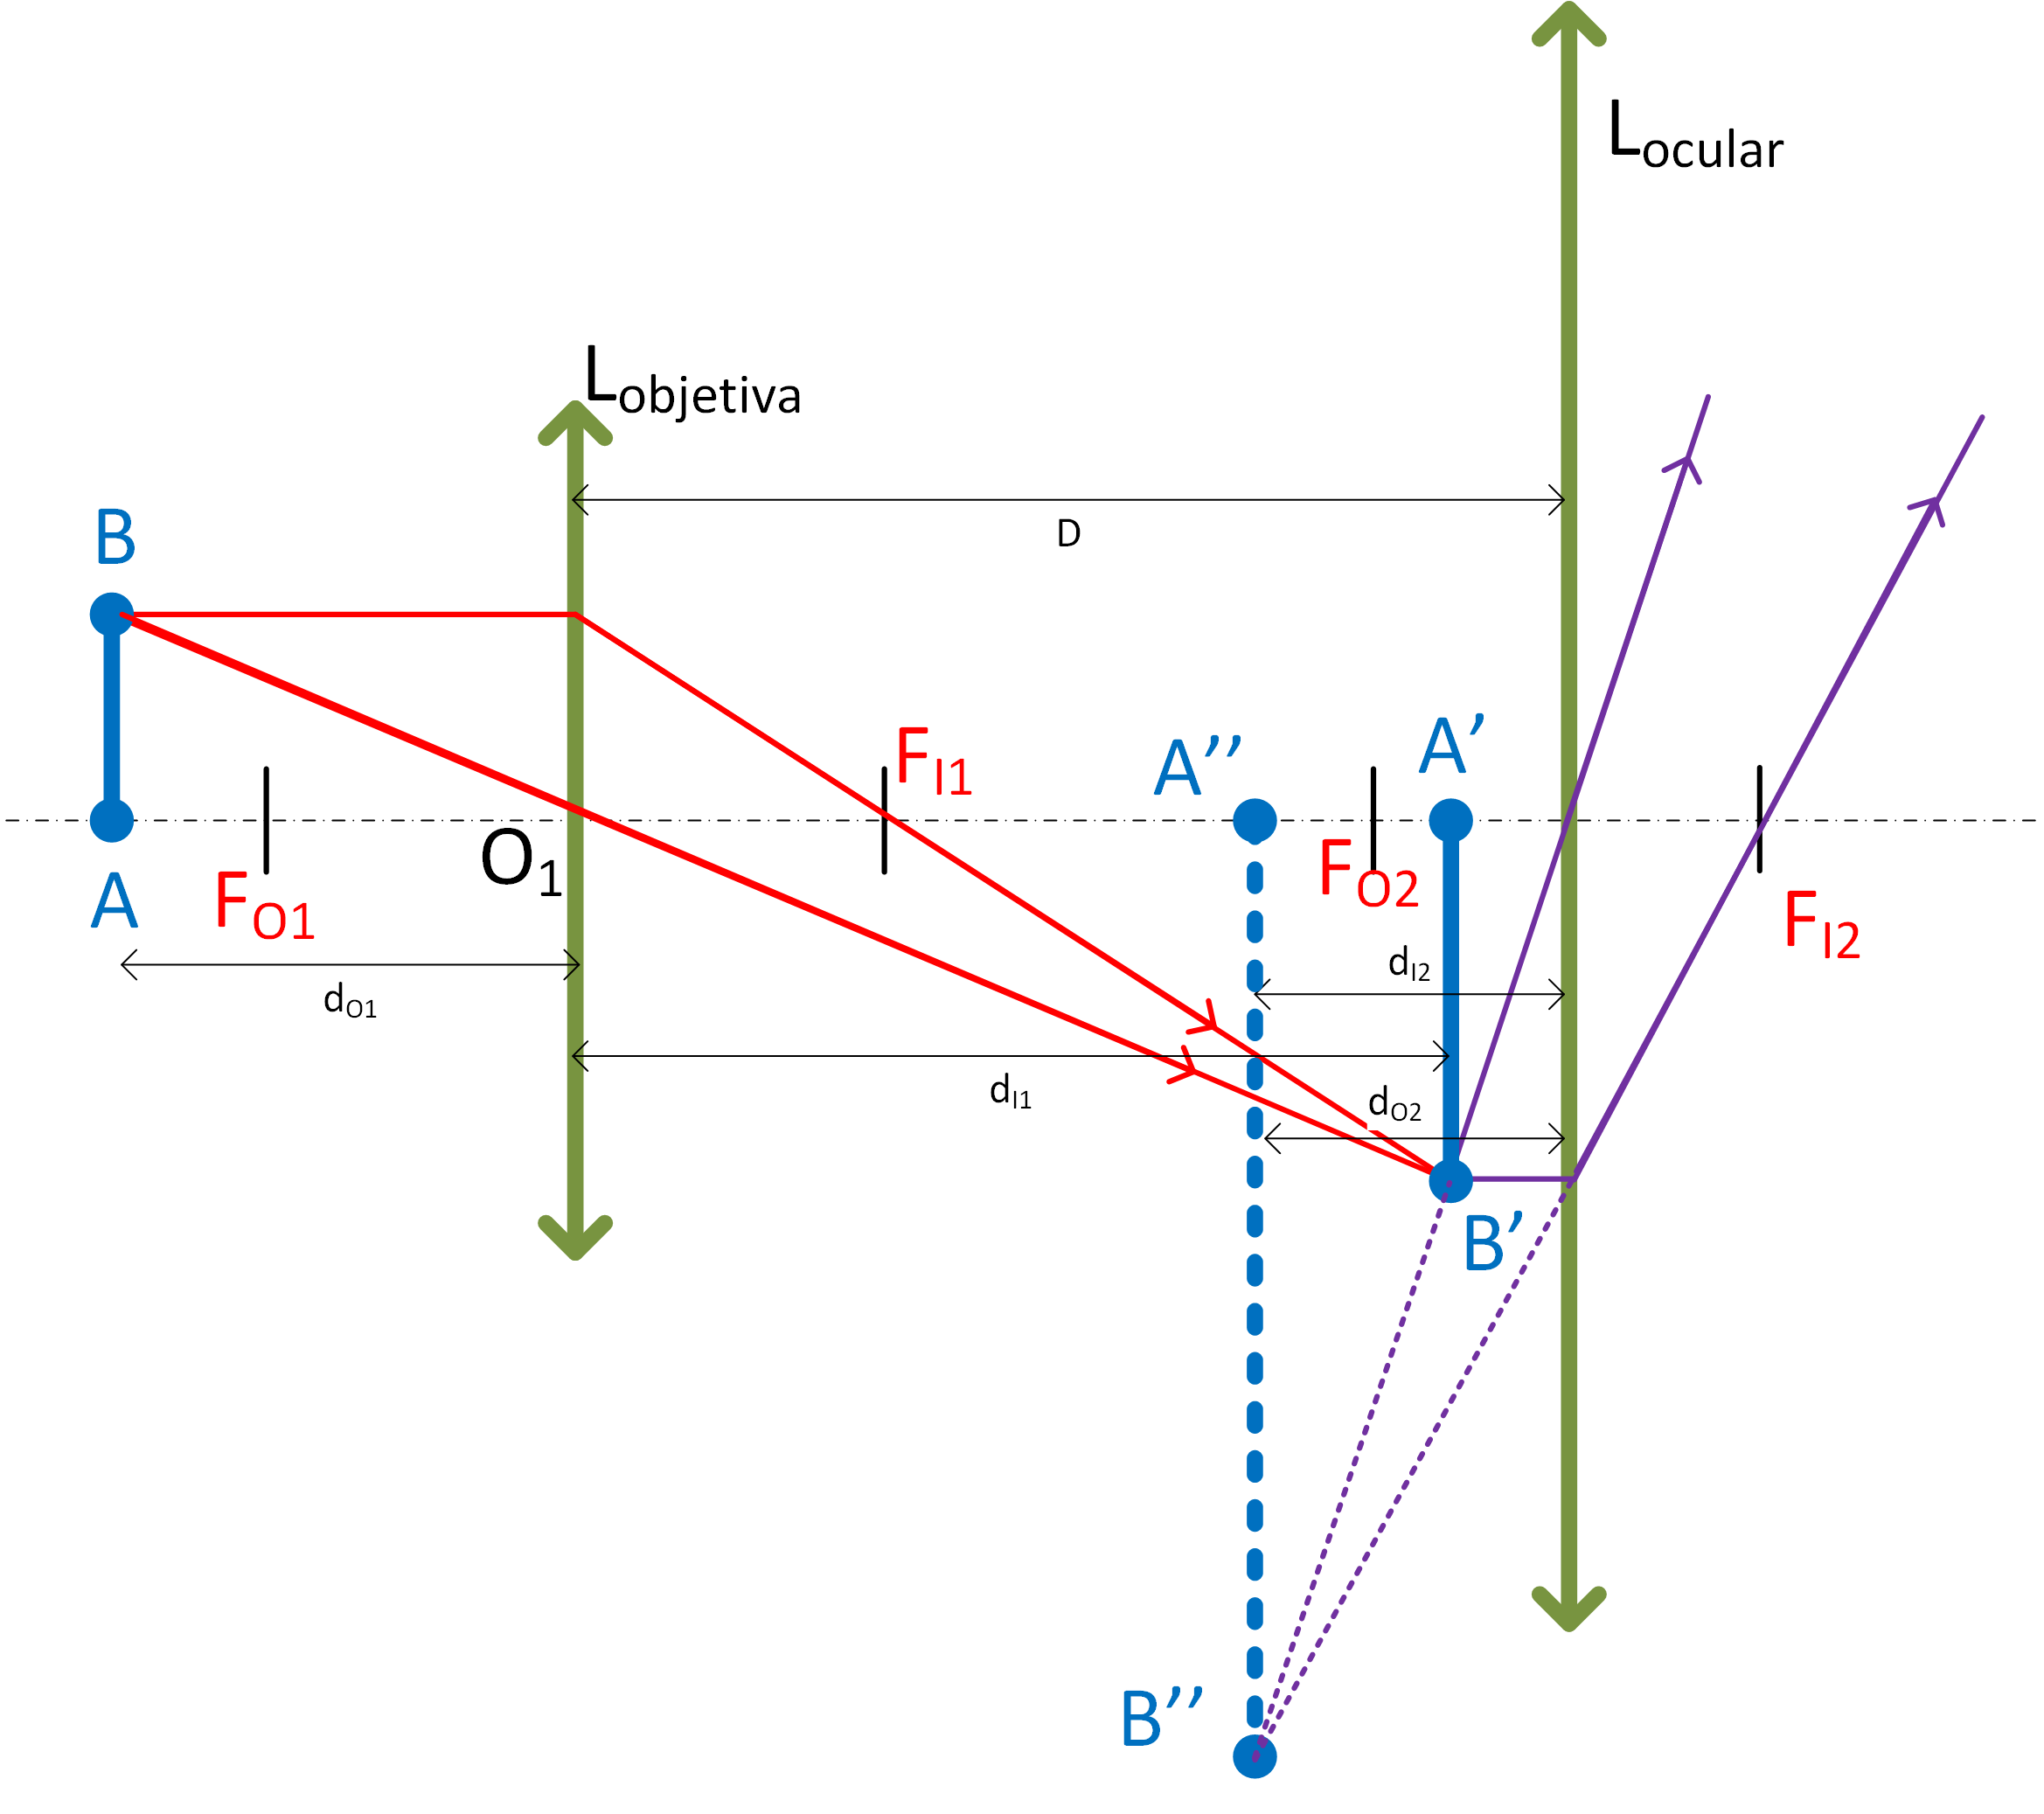
\includegraphics[width=0.6\textwidth]{Telescopio}
	\caption{Sistema ótico Microscópio/Telescópio. \label{fig:Telescopio}} 
\end{figure}


Em ambos os casos a segunda lente (ocular) está mais próxima da da imagem intermédia formada pela objetiva e portanto a imagem final seja \emph{virtual}, ou seja, visível apenas através da lente.
A ocular permite ampliar a imagem intermédia, tal como um lupa amplia
um objeto.
 
 Continua-se neste trabalho a usar a análise da Ótica Gaussiana, paraxial ou de 1ª ordem.


Como segundo objectivo pretende-se que os alunos tomem conhecimento e aprendam a manusear e a tomar medidas corretamente  com um instrumento ótico de precisão, o Goniómetro (Figura \ref{fig:spectrometer}). Este instrumento permite medir ângulos de desvio, por reflexão ou refração de feixes de raios paralelos, com uma resolução inferior a um minuto de grau.

\subsection{\sf Goniómetro de Babinet}
O goniómetro é um instrumento que permite medir ângulos. O goniómetro de Babinet tem uma forma central quase cilíndrica (a base) com uma plataforma que roda em torno do eixo (vertical) da base e onde é colocado um prisma (ou uma rede de difração) (Figura \ref{fig:spectrometer}). O goniómetro vem equipado com dois elementos ópticos: um colimador e uma luneta, que estão ambos montados radialmente, o colimador fixo e a luneta podendo rodar em torno do eixo da base (Figura 4). As posições angulares da plataforma (e portanto do prisma) e da luneta podem ser lidas num limbo graduado por intermédio de nónios solidários, respetivamente com a plataforma e a luneta. Existem dois parafusos micrométricos, cada um associado a cada um dos nónios que permitem com facilidade regular e fazer leituras das posições angulares, com resolução de $30''$ (meio minuto).

\begin{figure}[htb]  
\centering 
	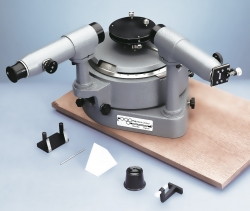
\includegraphics[width=0.45\textwidth]{spectrometer}
	\caption{Fotografia do goniómetro de Babinet (modelo Philipe Harris Advanced Spectrometer 30). \label{fig:spectrometer}} 
\end{figure}

O colimador, $C$, é constituído por dois tubos cilíndricos concêntricos que se podem deslocar axialmente. Um deles possui uma fenda retilínea, de largura variável por um parafuso, e que deve ser colocada na vertical (pode utiliara a mira da ocular depois de regulada). O outro tubo tem em posição oposta, i.e. mais próximo da região central, uma lente convergente, $L_C$. O objetivo deste conjunto, quando a fenda é iluminada por uma fonte luminosa divergente, é produzir um feixe de raios paralelos na região da plataforma, onde se coloca os prisma, rede, ou espelho. 
A fenda vai funcionar como objeto linear, se a fenda for relativamente estreita.

\begin{figure}[!htb]  
	\centering 
	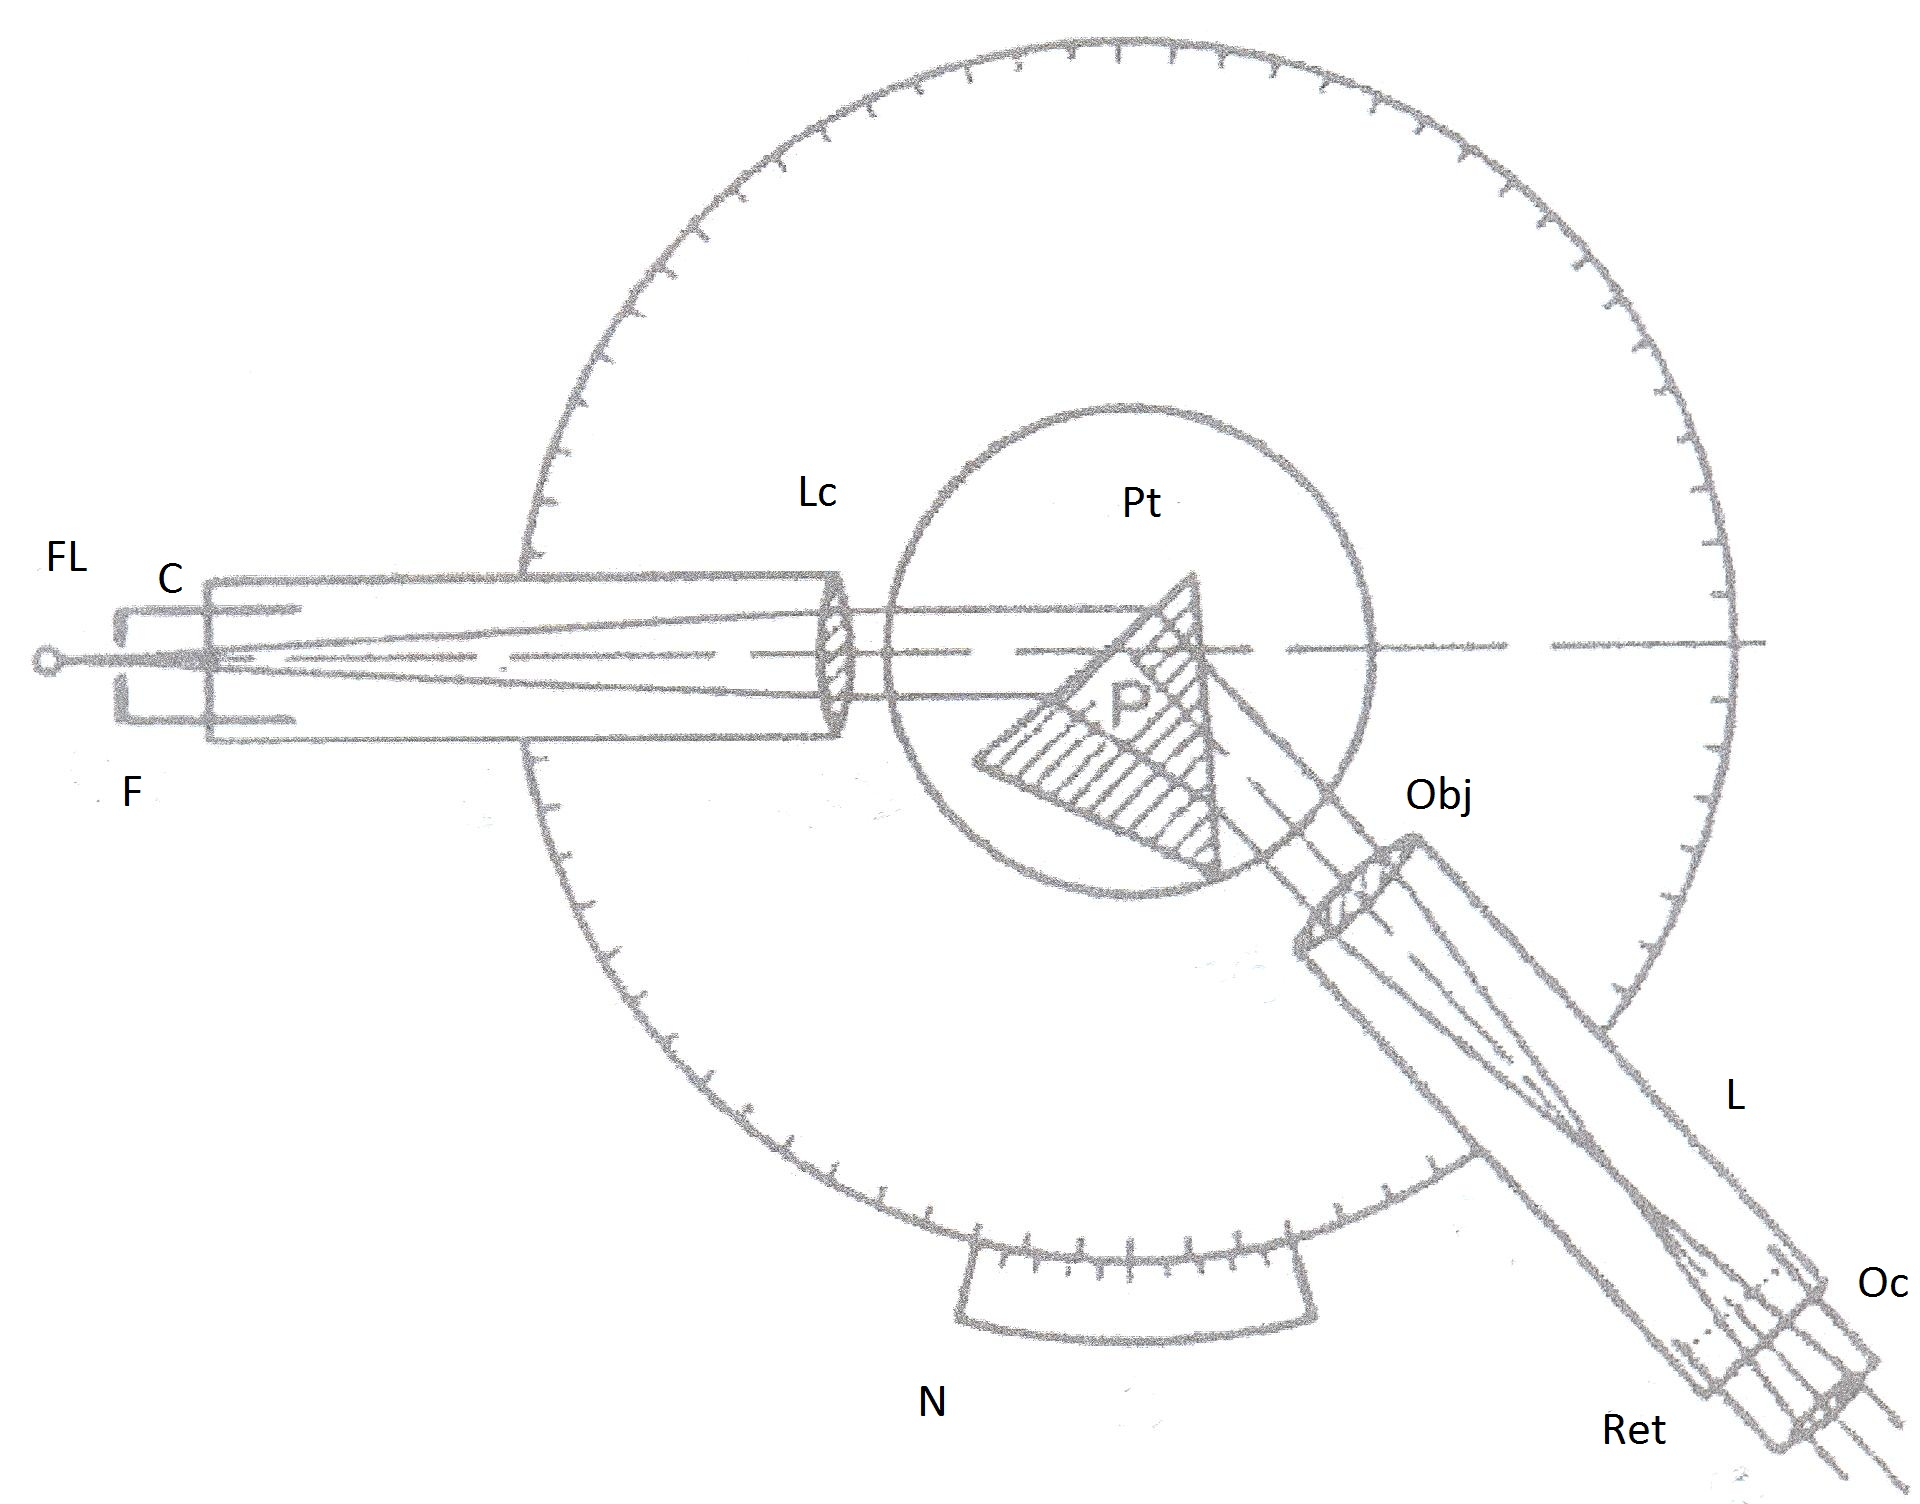
\includegraphics[width=0.65\textwidth]{babinet}
	\caption{Esquema do Goniómetro de Babinet. Legenda: FL-fonte luminosa, C-colimador, F-fenda, Lc-lente convergente do colimador, Pt-plataforma, P-Prisma, L-luneta, Obj-objetiva, Oc-ocular, Ret-retículo, N-nónio acoplado à luneta\label{fig:babinet}} 
\end{figure}

A luneta é constituída por dois elementos ópticos, uma lente convergente e uma ocular munida de retículo (dois fios cruzados perpendicularmente). A primeira lente produz no seu plano focal a imagem intemédia da fenda, que é projetada no plano do retículo e ampliada pela ocular. A ocular é regulada pelo observador, de modo a ver uma imagem focada da fenda. Quando se dispõe de um sistema de deteção (placa fotográfica ou um detetor, por exemplo uma célula fotoelétrica com um sistema de amplificação), este é colocado diretamente no plano focal da lente convergente e é retirada a ocular.
A regulação do Instrumento pelo utilizador é feita sempre na seguinte ordem:
\begin{enumerate}
\item Focar  o retículo para um olho sem necessidade de acomodação ( relaxado) e alinhá-lo com a vertical usar um fio de prumo, ou alguma linha vertical no Laboratório.
\item Focar a ocular observando um objecto no infinito (ou quase).
\item Alinhar a luneta e o colimador para observar a fenda iluminada. Focar a imagem da fenda, regulando APENAS o parafuso do colimador.
\item Alinhar fenda com a vertical, sobrepondo a mira e reduzir a sua largura para um valor suficientemente estreito, embora claramente visível.
\end{enumerate}

\subsection{\sf Questões a responder ANTES da sessão de Laboratório:}
\begin{enumerate}
\item Descreva por palavras suas quais os objectivos do Trabalho que irá realizar na sessão de Laboratório (uma folha A4). Indique as expressões que irá utilizar para obter as grandezas experimentais, bem como as expressões para calcular as incertezas. Inclua esta parte também no Relatório. Este irá constituir o ÚNICO meio de consulta na Prova Individual.
	
\item A partir da equação das lentes delgadas $\frac{1}{f} = (n_{vidro}-1) \left(\frac{1}{R_1} -\frac{1}{R_2}\right)$ e assumindo que os dois raios, $R_1$, $R_2$ das superfícies esféricas das lentes utilizadas no trabalho anterior são iguais e $ n_{vidro}=1.57$, calcule $R_{1,2}$ para todas as lentes esféricas utilizadas no trabalho de Ótica.
\item Assumindo que o diâmetro das lentes é $D=4cm$, calcule a espessura mínima da lentes. Podem ser finalmente ser consideradas como lentes delgadas?
\item Como variam as distâncias focais se estas lentes forem mergulhada em água?
\end{enumerate}

\subsection{\sf Material utilizado}
1ª Parte: Caixa de Óptica equipada com calha graduada, lentes convergentes e divergente, semi-cilindro de 
vidro acrílico, objeto com mira, diafragmas, suportes. 
Fonte luminosa com lâmpada de incandescência linear. 

2ª Parte: Goniómetro. Fonte de luz incandescente (candeiro). Luz expectral de $Hg$ ou $He$. Prisma. Rede de difração. Nível graduado.

\subsection{\sf Procedimento Experimental}

\subsubsection{\sf  Telescópio}

A montagem  a utilizar é da Figura \ref{fig:Telescopio}, embora o objecto estaja situa a uma distância grande ($> 5 \, m$). 


\begin{enumerate}
\item Na folha quadriculada em anexo desenhe um diagrama de traçado de raios utilizando como a lente objectiva a mais potente do trabalho de O.G.  e o objecto no infinito. Obtenha a posição da imagem intermédida(plano focal). Calcule agora a posição da lente ocular, com $f_{ocu}=150\,mm$, para obter uma ampliação transversal entre a Imagem intermédia e a Imagem final de $M_T=-3$. Utilizando as aproximações paraxial e das lentes delgadas desenhe a construção geométrica e obtenha a posição da imagem e a respetiva ampliação.
\item Tente montar o sistema na calha e observe um objeto distante a partir da lente ocular. Foque bem a imagem e registe a posição das duas lentes. Compare com o diagrama de traçado de raios.
%\item Calcule a o Número f do telecópio (inverso da Abertura %relativa)   a partir dos diâmetro, $D$, e distancia focal da %Objetiva, $f$. Compare com o valores das máquinas fotográficas %comerciais.
%$$f/\# \equiv \frac{}{}$$. 
\end{enumerate}

\subsubsection{\sf  Microscópio}

Nesta montagem equivalente iremos trocar a posição da lentes (objetiva/ocular) e colocar um pequeno objeto a uma distância um pouco maior do que a $f_{objetiva}$. 

A ampliação total deste sistema é o produto da ampliação transversal da objectiva, $M_{T_{obj}}$,  e da \emph{ampliação angular}\footnote{Definida como a razão entre a dimensão da imagem na retina quando o objeto é visto através da lente e a dimensão do objecto quando visto pelo olho desarmado à distância normal de observação, que é cerca de $25\,cm$}, da ocular, $M_{A_{ocu}}$ 
 
$M_{T_{obj}}$ é calculada pela razão:
$$M_{T_{obj}}=-d_I/d_O=-(d_I - f_{obj})/f_{obj}$$

A ampliação angular pode ser estimada por 
$$M_{A_{ocu}}= \frac{0.25}{f_{ocu}}$$

\begin{enumerate}
\item Na folha quadriculada em anexo desenhe um diagrama de traçado de raios, com o objecto a uma distância do foco $\equiv f/5$. Obtenha a posição da imagem intermédia. Calcule agora a posição da lente ocular para obter um feixe de raios paralelos (imagem no infinito)
\item Tente montar o sistema na calha e observe o slide com a mira graduada. Com auxílio do slide transparente graduado tente estimar a ampliação do  objeto distante a partir da lente ocular. Foque bem a imagem e registe a posição das duas lentes. Compare com o diagrama de traçado de raios.
\item Calcule a ampliação total do sistema.
\end{enumerate}

\subsubsection{\sf Goniómetro de Babinet}

\begin{enumerate}
%\item Ligue  a  lâmpada  espetral  e  espere  10  a  15  minutos    %até  que  se  estabeleça  o 
%equilíbrio térmico no seu interior. 
\item Disponha o Goniómtro em frente a uma fonte luminosa de luz incandescente.
\item Começe por regular a ocular da luneta do goniómetro. Para isso deve ver nitidamente com um 
olho  os fios do retículo e simultaneamente com o outro olho, ver um objeto no exterior da luneta afastado a cerca de 
$30\,cm$.  
\item Para  regular  a  objetiva,  observe  agora  um  objeto  no  “infinito” (no  laboratório 
escolha  um objeto  mais  afastado possível)  atuando  sobre  o  parafuso  da  luneta.  Regule  de  modo  a 
observar o objeto e o retículo bem focado e sem paralaxe. 
\item Coloque  a  luneta  alinhada de frente  do  colimador  e  regule  parafuso  do 
colimador de modo a observar a fenda focada quando iluminada pela lâmpada espetral. 
\item Verifique o nivelamento horizontal do goniómetro e da plataforma onde vai colocar o prisma com a ajuda de um nível de bolha. 
\item Identifique as escalas dos ângulos, para medir a posição da palataforma e da luneta. Como estão relacionadas as duas escalas opostas. Qual a resolução mínima do conjunto escala/nónio?
\item Observe a reflexão em cada face que define o ângulo do prisma e registe a posição angular 
correspondente a essas reflexões. Cada observador deve fazer três determinações usando o 
parafuso  micrométrico e centrando  a  imagem  da  fenda  com  o retículo  por  aproximação  à direita e à esquerda. Calcule o ângulo principal entre as duas faces polidas do prisma através desta medição.
\item Substitua no centro da plataforma do goniómetro o prisma por uma rede de difração de 
600 linhas por milímetro e a fonte por uma luz espectral (lâmpada de mercúrio ou Hélio). Observe os raios \emph{difratados} de várias cõres, de 1ª e 2ª ordem. Tende medir os ângulos de desvio, com a melhor precisão possível.

\end{enumerate}


	
\newpage
\def\width{18}
\def\hauteur{25}
\begin{tikzpicture}[x=1cm, y=1cm, semitransparent]
\draw[step=1mm, line width=0.1mm, black!30!white] (0,0) grid (\width,\hauteur);
\draw[step=5mm, line width=0.2mm, black!40!white] (0,0) grid (\width,\hauteur);
\draw[step=5cm, line width=0.5mm, black!50!white] (0,0) grid (\width,\hauteur);
\draw[step=1cm, line width=0.3mm, black!90!white] (0,0) grid (\width,\hauteur);
\end{tikzpicture}

\newpage
\def\width{18}
\def\hauteur{25}
\begin{tikzpicture}[x=1cm, y=1cm, semitransparent]
\draw[step=1mm, line width=0.1mm, black!30!white] (0,0) grid (\width,\hauteur);
\draw[step=5mm, line width=0.2mm, black!40!white] (0,0) grid (\width,\hauteur);
\draw[step=5cm, line width=0.5mm, black!50!white] (0,0) grid (\width,\hauteur);
\draw[step=1cm, line width=0.3mm, black!90!white] (0,0) grid (\width,\hauteur);
\end{tikzpicture}

\end{document} 